\documentclass[12pt, a4paper]{article}
\usepackage{fullpage}
\usepackage[T1]{fontenc}
\usepackage{multicol}
\usepackage{amsmath}
\numberwithin{figure}{subsection}
\numberwithin{table}{subsection}
\usepackage{listings}
\lstset{
  language=Java,
  basicstyle=\ttfamily\small,
  keywordstyle=\color{blue}\bfseries,
  commentstyle=\color{gray},
  stringstyle=\color{green!50!black},
  breaklines=true,
  numberstyle=\tiny,
  frame=single,
  captionpos=b
}
\usepackage{array}
\usepackage{enumitem}
\usepackage{graphicx}
\usepackage{float}
\usepackage{adjustbox}
\usepackage{xcolor}
\usepackage{caption}
\usepackage{pgfplots}
\pgfplotsset{compat=1.18}
\usepackage{pgfplotstable}
\usepackage{hyperref}
\hypersetup{
    colorlinks=true,
    linkcolor=black,
    filecolor=black,      
    urlcolor=black,
    pdftitle={Rozproszony bufor w JCSP},
    pdfauthor={Jan Gawroński},
    pdfpagemode=FullScreen,
    }

\title{\huge{Rozproszony bufor w JCSP}}
\date{09.12.2025}

\begin{document}
    \maketitle
    \section{Schemat połączeń}
      \begin{figure}[H]
      \centering
          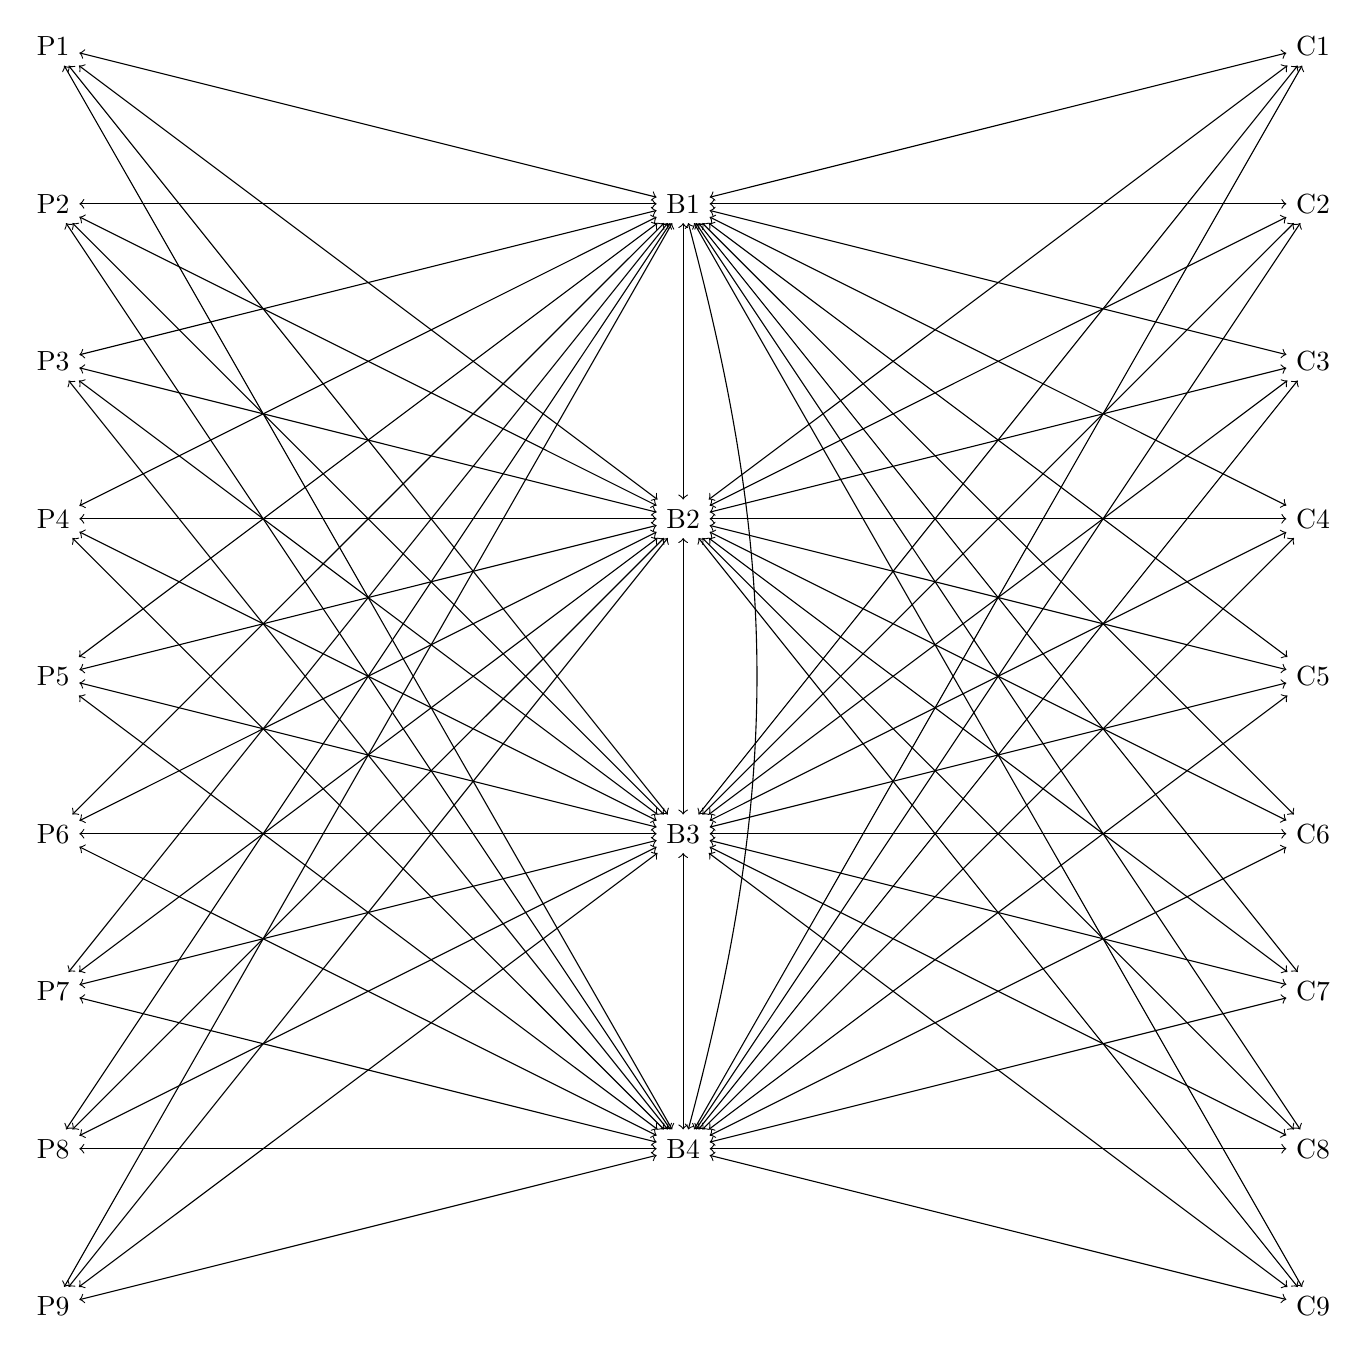
\begin{tikzpicture}[<->,scale=8]
              \node (C1) at ( 1, 1)     {C1};
              \node (C2) at ( 1, 0.75)  {C2};
              \node (C3) at ( 1, 0.5)   {C3};
              \node (C4) at ( 1, 0.25)  {C4};
              \node (C5) at ( 1, -0.0)  {C5};
              \node (C6) at ( 1, -0.25) {C6};
              \node (C7) at ( 1, -0.5)  {C7};
              \node (C8) at ( 1, -0.75) {C8};
              \node (C9) at ( 1, -1)    {C9};
              \node (P1) at (-1, 1)     {P1};
              \node (P2) at (-1, 0.75)  {P2};
              \node (P3) at (-1, 0.5)   {P3};
              \node (P4) at (-1, 0.25)  {P4};
              \node (P5) at (-1, -0.0)  {P5};
              \node (P6) at (-1, -0.25) {P6};
              \node (P7) at (-1, -0.5)  {P7};
              \node (P8) at (-1, -0.75) {P8};
              \node (P9) at (-1, -1)    {P9};
              \node (B1) at ( 0, 0.75)  {B1};
              \node (B2) at ( 0, 0.25)  {B2};
              \node (B3) at ( 0, -0.25) {B3};
              \node (B4) at ( 0, -0.75) {B4};
                      
              \path (P1) edge node {} (B1);
              \path (P2) edge node {} (B1);
              \path (P3) edge node {} (B1);
              \path (P4) edge node {} (B1);
              \path (P5) edge node {} (B1);
              \path (P6) edge node {} (B1);
              \path (P7) edge node {} (B1);
              \path (P8) edge node {} (B1);
              \path (P9) edge node {} (B1);
              \path (P1) edge node {} (B2);
              \path (P2) edge node {} (B2);
              \path (P3) edge node {} (B2);
              \path (P4) edge node {} (B2);
              \path (P5) edge node {} (B2);
              \path (P6) edge node {} (B2);
              \path (P7) edge node {} (B2);
              \path (P8) edge node {} (B2);
              \path (P9) edge node {} (B2);
              \path (P1) edge node {} (B3);
              \path (P2) edge node {} (B3);
              \path (P3) edge node {} (B3);
              \path (P4) edge node {} (B3);
              \path (P5) edge node {} (B3);
              \path (P6) edge node {} (B3);
              \path (P7) edge node {} (B3);
              \path (P8) edge node {} (B3);
              \path (P9) edge node {} (B3);
              \path (P1) edge node {} (B4);
              \path (P2) edge node {} (B4);
              \path (P3) edge node {} (B4);
              \path (P4) edge node {} (B4);
              \path (P5) edge node {} (B4);
              \path (P6) edge node {} (B4);
              \path (P7) edge node {} (B4);
              \path (P8) edge node {} (B4);
              \path (P9) edge node {} (B4);

              \path (C1) edge node {} (B1);
              \path (C2) edge node {} (B1);
              \path (C3) edge node {} (B1);
              \path (C4) edge node {} (B1);
              \path (C5) edge node {} (B1);
              \path (C6) edge node {} (B1);
              \path (C7) edge node {} (B1);
              \path (C8) edge node {} (B1);
              \path (C9) edge node {} (B1);
              \path (C1) edge node {} (B2);
              \path (C2) edge node {} (B2);
              \path (C3) edge node {} (B2);
              \path (C4) edge node {} (B2);
              \path (C5) edge node {} (B2);
              \path (C6) edge node {} (B2);
              \path (C7) edge node {} (B2);
              \path (C8) edge node {} (B2);
              \path (C9) edge node {} (B2);
              \path (C1) edge node {} (B3);
              \path (C2) edge node {} (B3);
              \path (C3) edge node {} (B3);
              \path (C4) edge node {} (B3);
              \path (C5) edge node {} (B3);
              \path (C6) edge node {} (B3);
              \path (C7) edge node {} (B3);
              \path (C8) edge node {} (B3);
              \path (C9) edge node {} (B3);
              \path (C1) edge node {} (B4);
              \path (C2) edge node {} (B4);
              \path (C3) edge node {} (B4);
              \path (C4) edge node {} (B4);
              \path (C5) edge node {} (B4);
              \path (C6) edge node {} (B4);
              \path (C7) edge node {} (B4);
              \path (C8) edge node {} (B4);
              \path (C9) edge node {} (B4);

              \path (B1) edge node {} (B2);
              \path (B2) edge node {} (B3);
              \path (B3) edge node {} (B4);
              \path (B4) edge[bend right=15] node {} (B1);
          \end{tikzpicture}
      \end{figure}

    \section{Implementacja}
      \subsection{Bufor}
        \lstinputlisting{QueueBuffer.java}
      \subsection{Producent}
        \lstinputlisting{QueueProducer.java}
      \subsection{Konsument}
        \lstinputlisting{QueueConsumer.java}
    
    \section{Wyniki testu równoważenia obciążenia}

    \subsection{10 producentów, 10 konsumentów, 10 buforów, 20 wielkość bufora}

    \begin{figure}[H]
      \centering
      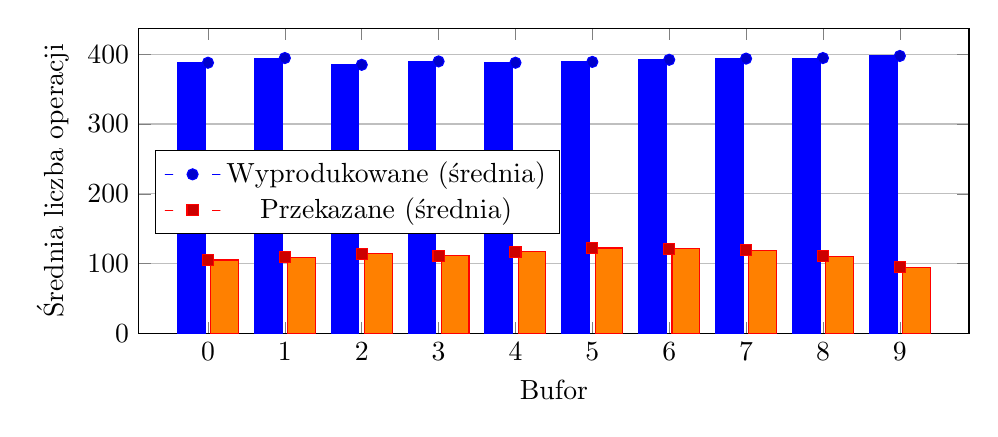
\begin{tikzpicture}
        \begin{axis}[
          width=\textwidth, height=0.45\textwidth,
          symbolic x coords={0,1,2,3,4,5,6,7,8,9},
          xtick=data,
          xlabel={Bufor},
          ylabel={Średnia liczba operacji},
          ymajorgrids=true,
          ymin=0,
          bar width=10pt,
          legend style={at={(0.02,0.6)},anchor=north west}
        ]
          \addplot+[ybar,fill=blue,bar shift=-6pt] coordinates {
            (0, 387.90) (1, 394.60) (2, 384.90) (3, 389.80) (4, 387.90) (5, 389.10) (6, 392.10) (7, 393.80) (8, 394.60) (9, 397.60)   
          };
          \addplot+[ybar,fill=orange,bar shift=6pt] coordinates {
            (0, 105.10) (1, 109.20) (2, 114.30) (3, 111.40) (4, 116.80) (5, 122.30) (6, 121.00) (7, 119.30) (8, 110.70) (9, 94.90)
          };
          \legend{Wyprodukowane (średnia), Przekazane (średnia)}
        \end{axis}
      \end{tikzpicture}
      \caption{Producenci - wyprodukowe, a przekazane}
    \end{figure}

    \begin{figure}[H]
      \centering
      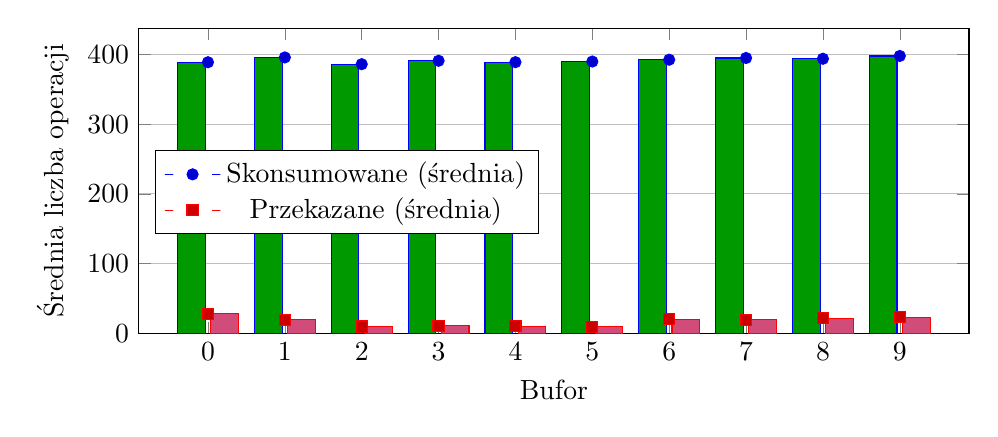
\begin{tikzpicture}
        \begin{axis}[
          width=\textwidth, height=0.45\textwidth,
          symbolic x coords={0,1,2,3,4,5,6,7,8,9},
          xtick=data,
          xlabel={Bufor},
          ylabel={Średnia liczba operacji},
          ymajorgrids=true,
          ymin=0,
          bar width=10pt,
          legend style={at={(0.02,0.6)},anchor=north west}
        ]
          \addplot+[ybar,fill=green!60!black,bar shift=-6pt] coordinates {
            (0, 388.70) (1, 395.60) (2, 385.90) (3, 390.80) (4, 388.80) (5, 389.70) (6, 392.30) (7, 394.80) (8, 393.70) (9, 397.70) 
          };
          \addplot+[ybar,fill=purple!70,bar shift=6pt] coordinates {
            (0, 28.20) (1, 19.70) (2, 9.70) (3, 10.60) (4, 10.10) (5, 9.50) (6, 20.20) (7, 19.70) (8, 21.40) (9, 23.10)   
          };
          \legend{Skonsumowane (średnia), Przekazane (średnia)}
        \end{axis}
      \end{tikzpicture}
      \caption{Konsumenci - skonsumowane, a przekazane}
    \end{figure}

    \begin{figure}[H]
      \centering
      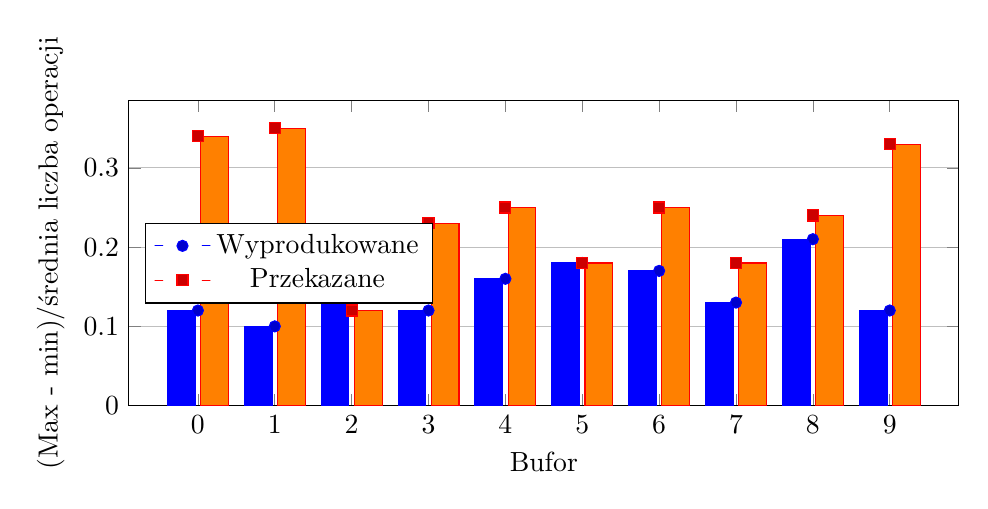
\begin{tikzpicture}
        \begin{axis}[
          width=\textwidth, height=0.45\textwidth,
          symbolic x coords={0,1,2,3,4,5,6,7,8,9},
          xtick=data,
          xlabel={Bufor},
          ylabel={(Max - min)/średnia liczba operacji},
          ymajorgrids=true,
          ymin=0,
          bar width=10pt,
          legend style={at={(0.02,0.6)},anchor=north west}
        ]
          \addplot+[ybar,fill=blue,bar shift=-6pt] coordinates {
            (0, 0.12) (1, 0.10) (2, 0.16) (3, 0.12) (4, 0.16) (5, 0.18) (6, 0.17) (7, 0.13) (8, 0.21) (9, 0.12) 
          };
          \addplot+[ybar,fill=orange,bar shift=6pt] coordinates {
            (0, 0.34) (1, 0.35) (2, 0.12) (3, 0.23) (4, 0.25) (5, 0.18) (6, 0.25) (7, 0.18) (8, 0.24) (9, 0.33) 
          };
          \legend{Wyprodukowane, Przekazane}
        \end{axis}
      \end{tikzpicture}
      \caption{Producenci - wyprodukowe, a przekazane ((Max - min)/średnia)}
    \end{figure}

    \begin{figure}[H]
      \centering
      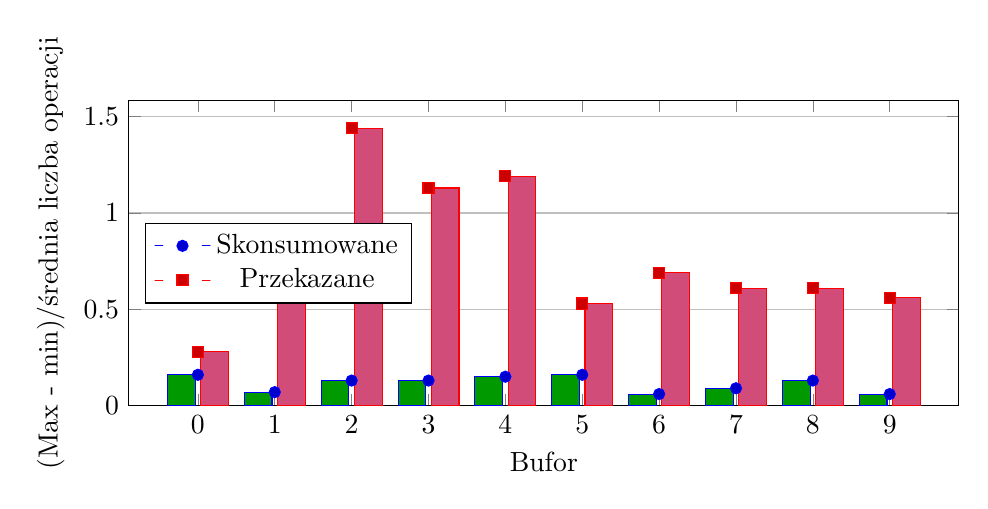
\begin{tikzpicture}
        \begin{axis}[
          width=\textwidth, height=0.45\textwidth,
          symbolic x coords={0,1,2,3,4,5,6,7,8,9},
          xtick=data,
          xlabel={Bufor},
          ylabel={(Max - min)/średnia liczba operacji},
          ymajorgrids=true,
          ymin=0,
          bar width=10pt,
          legend style={at={(0.02,0.6)},anchor=north west}
        ]
          \addplot+[ybar,fill=green!60!black,bar shift=-6pt] coordinates {
            (0, 0.16) (1, 0.07) (2, 0.13) (3, 0.13) (4, 0.15) (5, 0.16) (6, 0.06) (7, 0.09) (8, 0.13) (9, 0.06) 
          };
          \addplot+[ybar,fill=purple!70,bar shift=6pt] coordinates {
            (0, 0.28) (1, 0.86) (2, 1.44) (3, 1.13) (4, 1.19) (5, 0.53) (6, 0.69) (7, 0.61) (8, 0.61) (9, 0.56)
          };
          \legend{Skonsumowane, Przekazane}
        \end{axis}
      \end{tikzpicture}
      \caption{Konsumenci - skonsumowane, a przekazane (Max - min)/średnia}
    \end{figure}

    \subsection{10 producentów, 10 konsumentów, 10 buforów, 5 wielkość bufora}

    \begin{figure}[H]
      \centering
      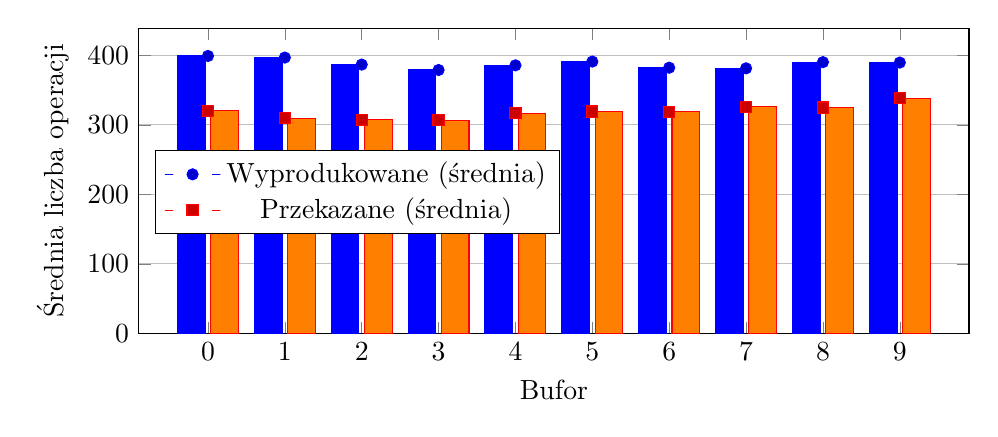
\begin{tikzpicture}
        \begin{axis}[
          width=\textwidth, height=0.45\textwidth,
          symbolic x coords={0,1,2,3,4,5,6,7,8,9},
          xtick=data,
          xlabel={Bufor},
          ylabel={Średnia liczba operacji},
          ymajorgrids=true,
          ymin=0,
          bar width=10pt,
          legend style={at={(0.02,0.6)},anchor=north west}
        ]
          \addplot+[ybar,fill=blue,bar shift=-6pt] coordinates {
            (0, 399.00) (1, 396.70) (2, 386.60) (3, 378.80) (4, 385.50) (5, 390.90) (6, 382.10) (7, 381.20) (8, 390.10) (9, 389.50) 
          };
          \addplot+[ybar,fill=orange,bar shift=6pt] coordinates {
            (0, 320.30) (1, 309.60) (2, 307.40) (3, 306.50) (4, 316.50) (5, 319.00) (6, 318.70) (7, 326.10) (8, 324.80) (9, 338.20) 
          };
          \legend{Wyprodukowane (średnia), Przekazane (średnia)}
        \end{axis}
      \end{tikzpicture}
      \caption{Producenci - wyprodukowe, a przekazane}
    \end{figure}

    \begin{figure}[H]
      \centering
      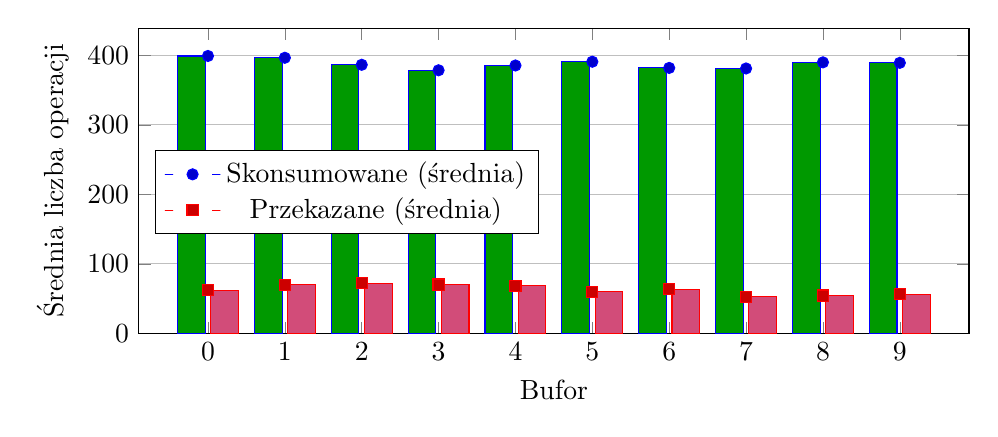
\begin{tikzpicture}
        \begin{axis}[
          width=\textwidth, height=0.45\textwidth,
          symbolic x coords={0,1,2,3,4,5,6,7,8,9},
          xtick=data,
          xlabel={Bufor},
          ylabel={Średnia liczba operacji},
          ymajorgrids=true,
          ymin=0,
          bar width=10pt,
          legend style={at={(0.02,0.6)},anchor=north west}
        ]
          \addplot+[ybar,fill=green!60!black,bar shift=-6pt] coordinates {
            (0, 399.10) (1, 396.50) (2, 386.40) (3, 378.50) (4, 385.40) (5, 390.80) (6, 381.90) (7, 381.10) (8, 389.90) (9, 389.20) 
          };
          \addplot+[ybar,fill=purple!70,bar shift=6pt] coordinates {
            (0, 62.00) (1, 70.10) (2, 71.90) (3, 70.20) (4, 68.40) (5, 60.00) (6, 63.70) (7, 52.60) (8, 54.40) (9, 56.30) 
          };
          \legend{Skonsumowane (średnia), Przekazane (średnia)}
        \end{axis}
      \end{tikzpicture}
      \caption{Konsumenci - skonsumowane, a przekazane}
    \end{figure}

    \begin{figure}[H]
      \centering
      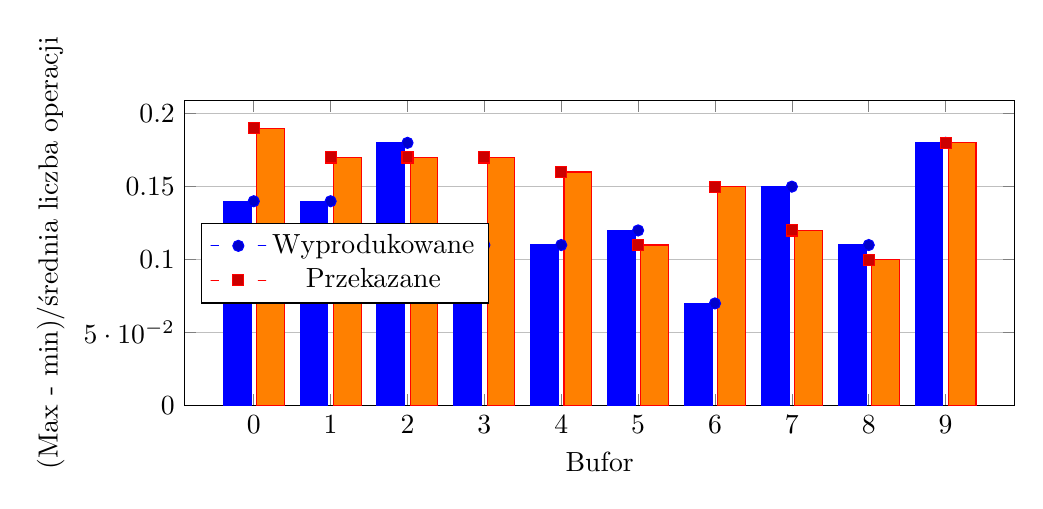
\begin{tikzpicture}
        \begin{axis}[
          width=\textwidth, height=0.45\textwidth,
          symbolic x coords={0,1,2,3,4,5,6,7,8,9},
          xtick=data,
          xlabel={Bufor},
          ylabel={(Max - min)/średnia liczba operacji},
          ymajorgrids=true,
          ymin=0,
          bar width=10pt,
          legend style={at={(0.02,0.6)},anchor=north west}
        ]
          \addplot+[ybar,fill=blue,bar shift=-6pt] coordinates {
            (0, 0.14) (1, 0.14) (2, 0.18) (3, 0.11) (4, 0.11) (5, 0.12) (6, 0.07) (7, 0.15) (8, 0.11) (9, 0.18) 
          };
          \addplot+[ybar,fill=orange,bar shift=6pt] coordinates {
            (0, 0.19) (1, 0.17) (2, 0.17) (3, 0.17) (4, 0.16) (5, 0.11) (6, 0.15) (7, 0.12) (8, 0.10) (9, 0.18) 
          };
          \legend{Wyprodukowane, Przekazane}
        \end{axis}
      \end{tikzpicture}
      \caption{Producenci - wyprodukowe, a przekazane ((Max - min)/średnia)}
    \end{figure}

    \begin{figure}[H]
      \centering
      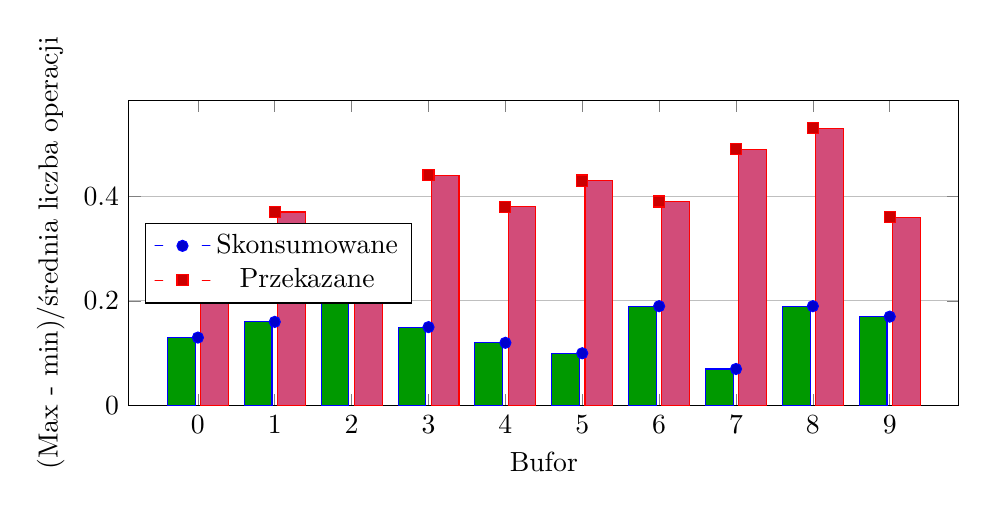
\begin{tikzpicture}
        \begin{axis}[
          width=\textwidth, height=0.45\textwidth,
          symbolic x coords={0,1,2,3,4,5,6,7,8,9},
          xtick=data,
          xlabel={Bufor},
          ylabel={(Max - min)/średnia liczba operacji},
          ymajorgrids=true,
          ymin=0,
          bar width=10pt,
          legend style={at={(0.02,0.6)},anchor=north west}
        ]
          \addplot+[ybar,fill=green!60!black,bar shift=-6pt] coordinates {
            (0, 0.13) (1, 0.16) (2, 0.22) (3, 0.15) (4, 0.12) (5, 0.10) (6, 0.19) (7, 0.07) (8, 0.19) (9, 0.17) 
          };
          \addplot+[ybar,fill=purple!70,bar shift=6pt] coordinates {
            (0, 0.32) (1, 0.37) (2, 0.28) (3, 0.44) (4, 0.38) (5, 0.43) (6, 0.39) (7, 0.49) (8, 0.53) (9, 0.36)                                                                                               
          };
          \legend{Skonsumowane, Przekazane}
        \end{axis}
      \end{tikzpicture}
      \caption{Konsumenci - skonsumowane, a przekazane (Max - min)/średnia}
    \end{figure}

    \subsection{10 producentów, 10 konsumentów, 5 buforów, 20 wielkość bufora}

    \begin{figure}[H]
      \centering
      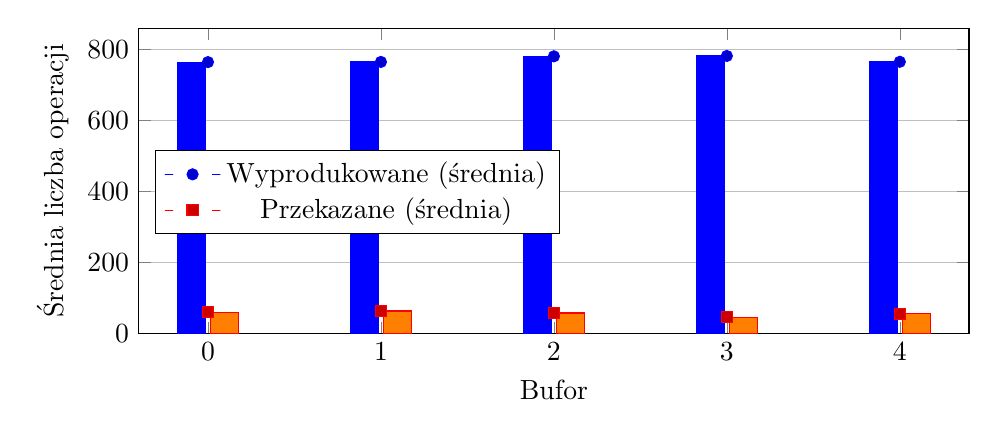
\begin{tikzpicture}
        \begin{axis}[
          width=\textwidth, height=0.45\textwidth,
          symbolic x coords={0,1,2,3,4},
          xtick=data,
          xlabel={Bufor},
          ylabel={Średnia liczba operacji},
          ymajorgrids=true,
          ymin=0,
          bar width=10pt,
          legend style={at={(0.02,0.6)},anchor=north west}
        ]
          \addplot+[ybar,fill=blue,bar shift=-6pt] coordinates {
            (0, 763.40) (1, 763.90) (2, 779.70) (3, 780.70) (4, 764.30) 
          };
          \addplot+[ybar,fill=orange,bar shift=6pt] coordinates {
            (0, 59.50) (1, 62.70) (2, 57.20) (3, 45.30) (4, 55.50) 
          };
          \legend{Wyprodukowane (średnia), Przekazane (średnia)}
        \end{axis}
      \end{tikzpicture}
      \caption{Producenci - wyprodukowe, a przekazane}
    \end{figure}

    \begin{figure}[H]
      \centering
      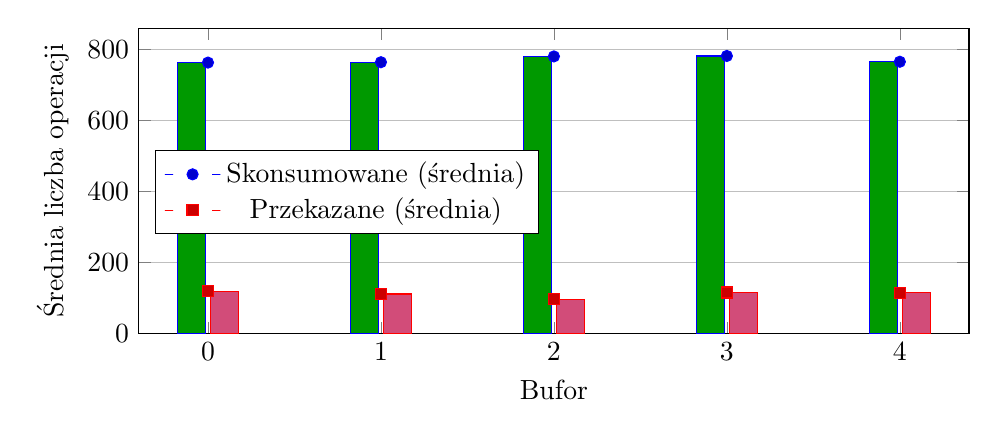
\begin{tikzpicture}
        \begin{axis}[
          width=\textwidth, height=0.45\textwidth,
          symbolic x coords={0,1,2,3,4},
          xtick=data,
          xlabel={Bufor},
          ylabel={Średnia liczba operacji},
          ymajorgrids=true,
          ymin=0,
          bar width=10pt,
          legend style={at={(0.02,0.6)},anchor=north west}
        ]
          \addplot+[ybar,fill=green!60!black,bar shift=-6pt] coordinates {
            (0, 762.80) (1, 763.90) (2, 780.20) (3, 781.50) (4, 765.20) 
          };
          \addplot+[ybar,fill=purple!70,bar shift=6pt] coordinates {
            (0, 119.10) (1, 110.80) (2, 96.00) (3, 115.10) (4, 113.80)
          };
          \legend{Skonsumowane (średnia), Przekazane (średnia)}
        \end{axis}
      \end{tikzpicture}
      \caption{Konsumenci - skonsumowane, a przekazane}
    \end{figure}

    \begin{figure}[H]
      \centering
      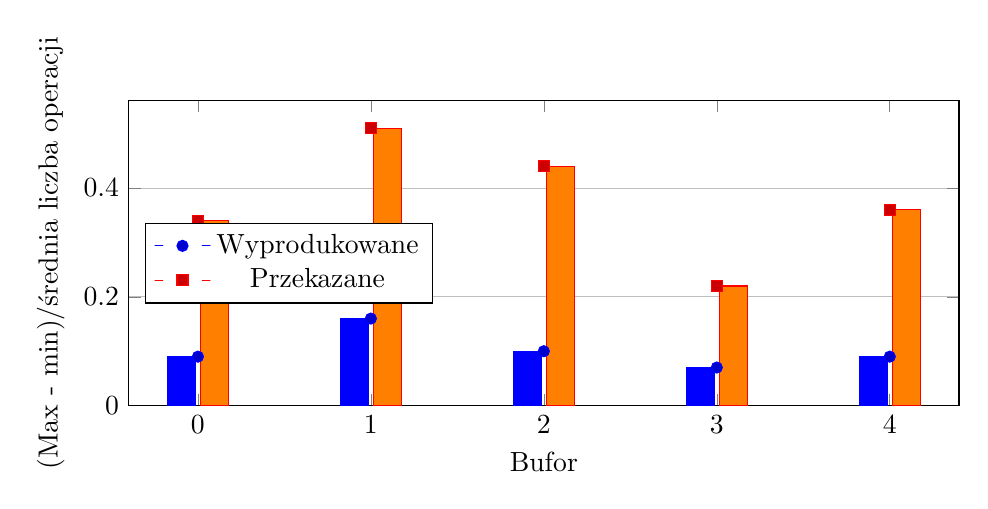
\begin{tikzpicture}
        \begin{axis}[
          width=\textwidth, height=0.45\textwidth,
          symbolic x coords={0,1,2,3,4},
          xtick=data,
          xlabel={Bufor},
          ylabel={(Max - min)/średnia liczba operacji},
          ymajorgrids=true,
          ymin=0,
          bar width=10pt,
          legend style={at={(0.02,0.6)},anchor=north west}
        ]
          \addplot+[ybar,fill=blue,bar shift=-6pt] coordinates {
            (0, 0.09) (1, 0.16) (2, 0.10) (3, 0.07) (4, 0.09) 
          };
          \addplot+[ybar,fill=orange,bar shift=6pt] coordinates {
            (0, 0.34) (1, 0.51) (2, 0.44) (3, 0.22) (4, 0.36) 
          };
          \legend{Wyprodukowane, Przekazane}
        \end{axis}
      \end{tikzpicture}
      \caption{Producenci - wyprodukowe, a przekazane ((Max - min)/średnia)}
    \end{figure}

    \begin{figure}[H]
      \centering
      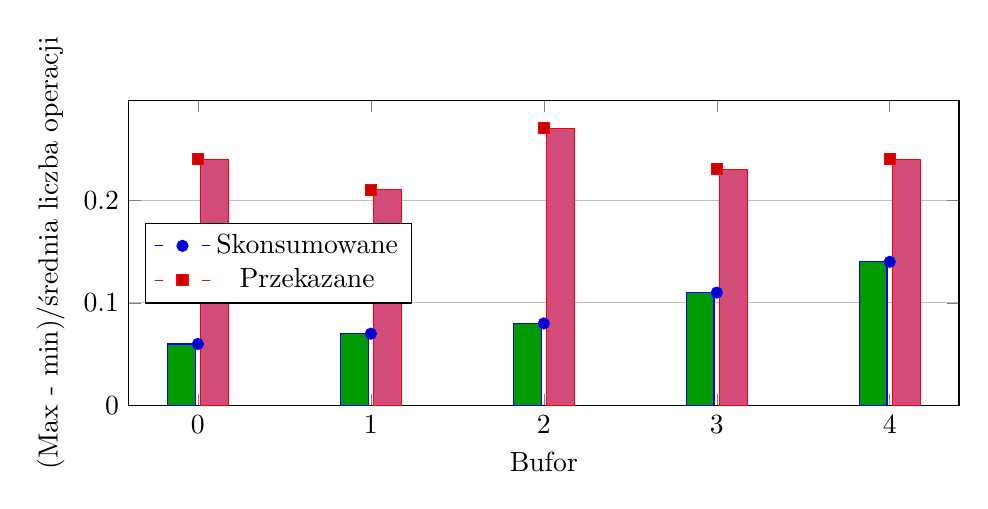
\begin{tikzpicture}
        \begin{axis}[
          width=\textwidth, height=0.45\textwidth,
          symbolic x coords={0,1,2,3,4},
          xtick=data,
          xlabel={Bufor},
          ylabel={(Max - min)/średnia liczba operacji},
          ymajorgrids=true,
          ymin=0,
          bar width=10pt,
          legend style={at={(0.02,0.6)},anchor=north west}
        ]
          \addplot+[ybar,fill=green!60!black,bar shift=-6pt] coordinates {
            (0, 0.06) (1, 0.07) (2, 0.08) (3, 0.11) (4, 0.14)
          };
          \addplot+[ybar,fill=purple!70,bar shift=6pt] coordinates {
            (0, 0.24) (1, 0.21) (2, 0.27) (3, 0.23) (4, 0.24)                                                                                              
          };
          \legend{Skonsumowane, Przekazane}
        \end{axis}
      \end{tikzpicture}
      \caption{Konsumenci - skonsumowane, a przekazane (Max - min)/średnia}
    \end{figure}

    \subsection{20 producentów, 10 konsumentów, 10 buforów, 20 wielkość bufora}

    \begin{figure}[H]
      \centering
      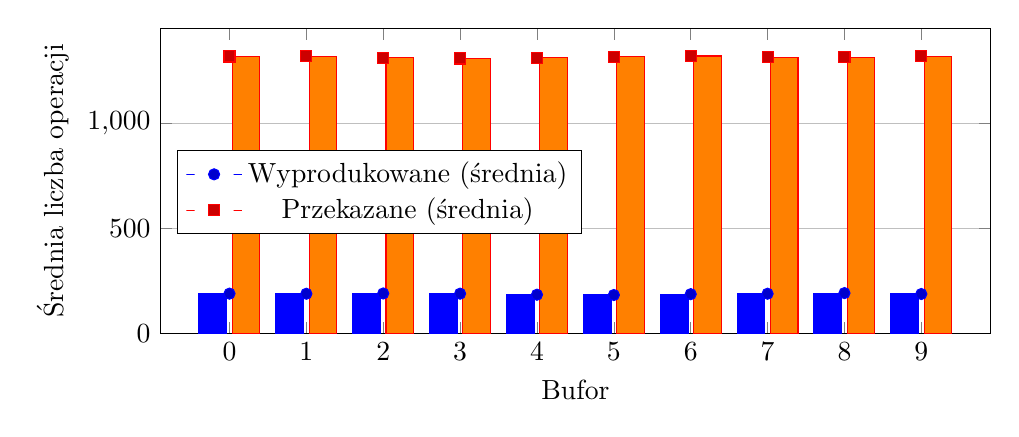
\begin{tikzpicture}
        \begin{axis}[
          width=\textwidth, height=0.45\textwidth,
          symbolic x coords={0,1,2,3,4,5,6,7,8,9},
          xtick=data,
          xlabel={Bufor},
          ylabel={Średnia liczba operacji},
          ymajorgrids=true,
          ymin=0,
          bar width=10pt,
          legend style={at={(0.02,0.6)},anchor=north west}
        ]
          \addplot+[ybar,fill=blue,bar shift=-6pt] coordinates {
            (0, 189.10) (1, 188.50) (2, 189.90) (3, 188.90) (4, 183.90) (5, 182.50) (6, 186.60) (7, 188.70) (8, 191.65) (9, 187.30) 
          };
          \addplot+[ybar,fill=orange,bar shift=6pt] coordinates {
            (0, 1318.95) (1, 1319.90) (2, 1312.50) (3, 1309.35) (4, 1313.50) (5, 1317.95) (6, 1321.35) (7, 1315.45) (8, 1314.90) (9, 1320.35) 
          };
          \legend{Wyprodukowane (średnia), Przekazane (średnia)}
        \end{axis}
      \end{tikzpicture}
      \caption{Producenci - wyprodukowe, a przekazane}
    \end{figure}

    \begin{figure}[H]
      \centering
      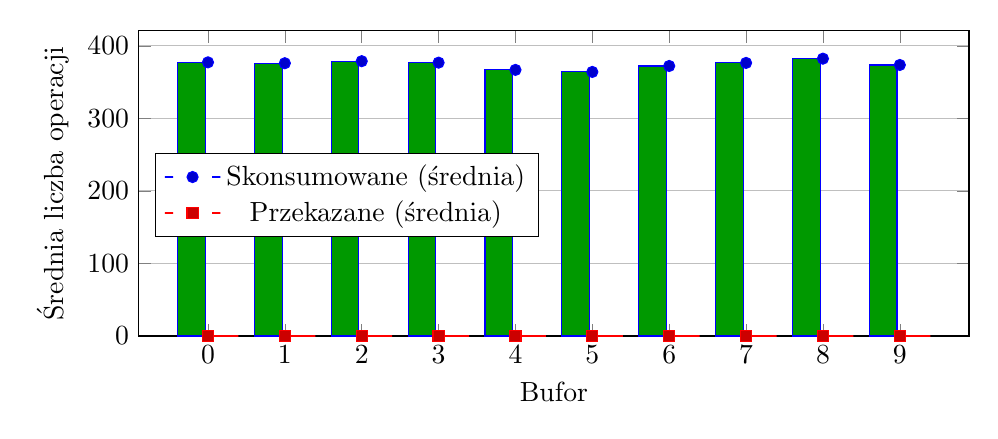
\begin{tikzpicture}
        \begin{axis}[
          width=\textwidth, height=0.45\textwidth,
          symbolic x coords={0,1,2,3,4,5,6,7,8,9},
          xtick=data,
          xlabel={Bufor},
          ylabel={Średnia liczba operacji},
          ymajorgrids=true,
          ymin=0,
          bar width=10pt,
          legend style={at={(0.02,0.6)},anchor=north west}
        ]
          \addplot+[ybar,fill=green!60!black,bar shift=-6pt] coordinates {
            (0, 377.20) (1, 376.00) (2, 378.80) (3, 376.80) (4, 366.80) (5, 364.00) (6, 372.20) (7, 376.40) (8, 382.30) (9, 373.60) 
          };
          \addplot+[ybar,fill=purple!70,bar shift=6pt] coordinates {
            (0, 0.00) (1, 0.00) (2, 0.00) (3, 0.00) (4, 0.00) (5, 0.00) (6, 0.00) (7, 0.00) (8, 0.00) (9, 0.00) 
          };
          \legend{Skonsumowane (średnia), Przekazane (średnia)}
        \end{axis}
      \end{tikzpicture}
      \caption{Konsumenci - skonsumowane, a przekazane}
    \end{figure}

    \begin{figure}[H]
      \centering
      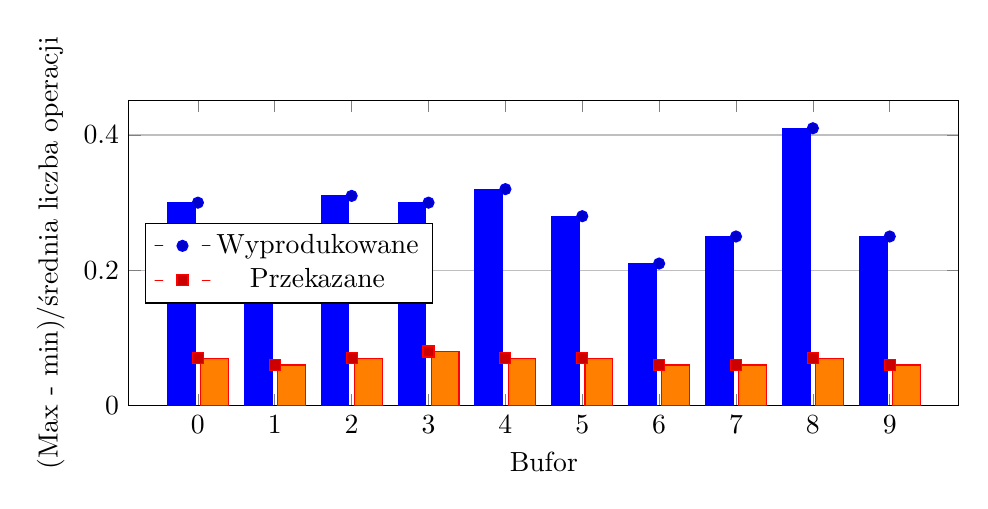
\begin{tikzpicture}
        \begin{axis}[
          width=\textwidth, height=0.45\textwidth,
          symbolic x coords={0,1,2,3,4,5,6,7,8,9},
          xtick=data,
          xlabel={Bufor},
          ylabel={(Max - min)/średnia liczba operacji},
          ymajorgrids=true,
          ymin=0,
          bar width=10pt,
          legend style={at={(0.02,0.6)},anchor=north west}
        ]
          \addplot+[ybar,fill=blue,bar shift=-6pt] coordinates {
            (0, 0.30) (1, 0.21) (2, 0.31) (3, 0.30) (4, 0.32) (5, 0.28) (6, 0.21) (7, 0.25) (8, 0.41) (9, 0.25) 
          };
          \addplot+[ybar,fill=orange,bar shift=6pt] coordinates {
            (0, 0.07) (1, 0.06) (2, 0.07) (3, 0.08) (4, 0.07) (5, 0.07) (6, 0.06) (7, 0.06) (8, 0.07) (9, 0.06) 
          };
          \legend{Wyprodukowane, Przekazane}
        \end{axis}
      \end{tikzpicture}
      \caption{Producenci - wyprodukowe, a przekazane ((Max - min)/średnia)}
    \end{figure}

    \begin{figure}[H]
      \centering
      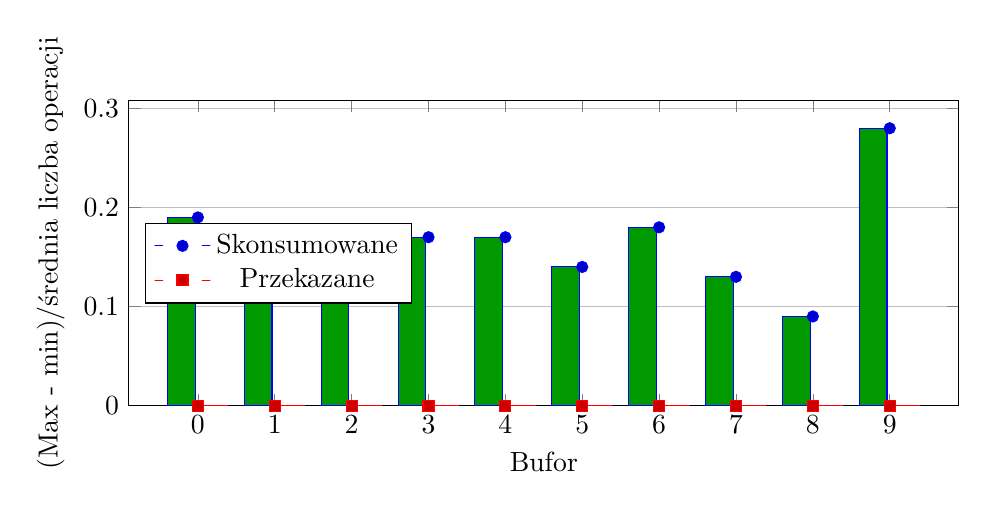
\begin{tikzpicture}
        \begin{axis}[
          width=\textwidth, height=0.45\textwidth,
          symbolic x coords={0,1,2,3,4,5,6,7,8,9},
          xtick=data,
          xlabel={Bufor},
          ylabel={(Max - min)/średnia liczba operacji},
          ymajorgrids=true,
          ymin=0,
          bar width=10pt,
          legend style={at={(0.02,0.6)},anchor=north west}
        ]
          \addplot+[ybar,fill=green!60!black,bar shift=-6pt] coordinates {
            (0, 0.19) (1, 0.15) (2, 0.15) (3, 0.17) (4, 0.17) (5, 0.14) (6, 0.18) (7, 0.13) (8, 0.09) (9, 0.28) 
          };
          \addplot+[ybar,fill=purple!70,bar shift=6pt] coordinates {
            (0, 0.00) (1, 0.00) (2, 0.00) (3, 0.00) (4, 0.00) (5, 0.00) (6, 0.00) (7, 0.00) (8, 0.00) (9, 0.00)                                                                                                                                                                                             
          };
          \legend{Skonsumowane, Przekazane}
        \end{axis}
      \end{tikzpicture}
      \caption{Konsumenci - skonsumowane, a przekazane (Max - min)/średnia}
    \end{figure}

    \subsection{10 producentów, 20 konsumentów, 10 buforów, 20 wielkość bufora}

    \begin{figure}[H]
      \centering
      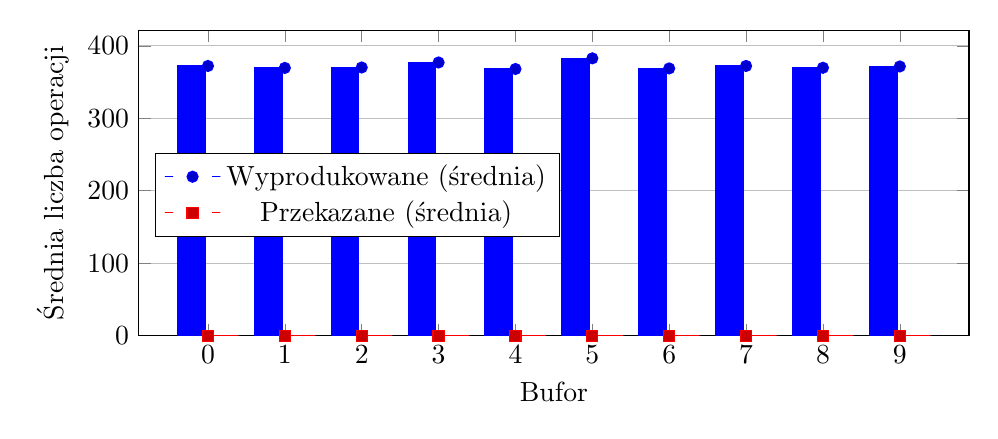
\begin{tikzpicture}
        \begin{axis}[
          width=\textwidth, height=0.45\textwidth,
          symbolic x coords={0,1,2,3,4,5,6,7,8,9},
          xtick=data,
          xlabel={Bufor},
          ylabel={Średnia liczba operacji},
          ymajorgrids=true,
          ymin=0,
          bar width=10pt,
          legend style={at={(0.02,0.6)},anchor=north west}
        ]
          \addplot+[ybar,fill=blue,bar shift=-6pt] coordinates {
            (0, 372.20) (1, 369.50) (2, 370.10) (3, 377.00) (4, 368.00) (5, 382.70) (6, 368.80) (7, 372.20) (8, 369.70) (9, 371.50) 
          };
          \addplot+[ybar,fill=orange,bar shift=6pt] coordinates {
            (0, 0.00) (1, 0.00) (2, 0.00) (3, 0.00) (4, 0.00) (5, 0.00) (6, 0.00) (7, 0.00) (8, 0.00) (9, 0.00) 
          };
          \legend{Wyprodukowane (średnia), Przekazane (średnia)}
        \end{axis}
      \end{tikzpicture}
      \caption{Producenci - wyprodukowe, a przekazane}
    \end{figure}

    \begin{figure}[H]
      \centering
      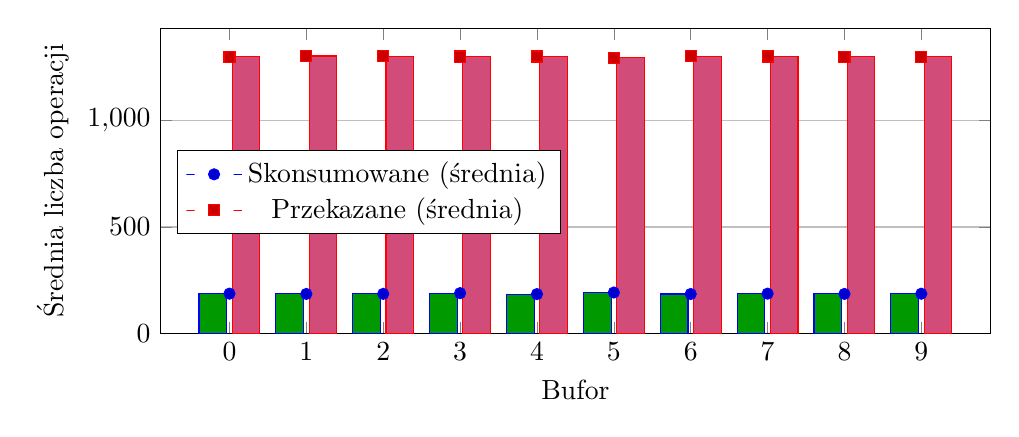
\begin{tikzpicture}
        \begin{axis}[
          width=\textwidth, height=0.45\textwidth,
          symbolic x coords={0,1,2,3,4,5,6,7,8,9},
          xtick=data,
          xlabel={Bufor},
          ylabel={Średnia liczba operacji},
          ymajorgrids=true,
          ymin=0,
          bar width=10pt,
          legend style={at={(0.02,0.6)},anchor=north west}
        ]
          \addplot+[ybar,fill=green!60!black,bar shift=-6pt] coordinates {
           (0, 186.60) (1, 185.25) (2, 185.55) (3, 189.00) (4, 184.50) (5, 191.85) (6, 184.90) (7, 186.60) (8, 185.35) (9, 186.25) 
          };
          \addplot+[ybar,fill=purple!70,bar shift=6pt] coordinates {
            (0, 1299.55) (1, 1304.15) (2, 1303.35) (3, 1301.45) (4, 1301.55) (5, 1295.85) (6, 1303.40) (7, 1301.95) (8, 1299.85) (9, 1300.55) 
          };
          \legend{Skonsumowane (średnia), Przekazane (średnia)}
        \end{axis}
      \end{tikzpicture}
      \caption{Konsumenci - skonsumowane, a przekazane}
    \end{figure}

    \begin{figure}[H]
      \centering
      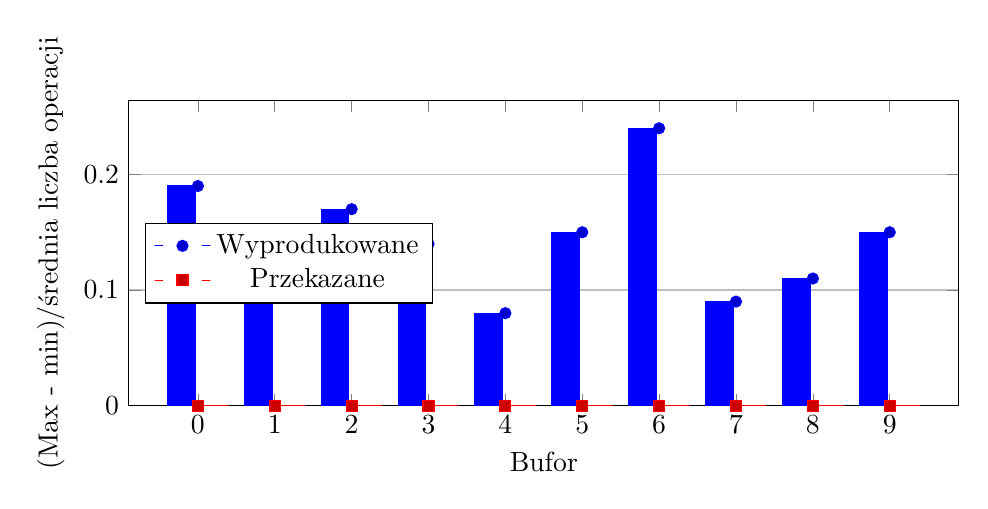
\begin{tikzpicture}
        \begin{axis}[
          width=\textwidth, height=0.45\textwidth,
          symbolic x coords={0,1,2,3,4,5,6,7,8,9},
          xtick=data,
          xlabel={Bufor},
          ylabel={(Max - min)/średnia liczba operacji},
          ymajorgrids=true,
          ymin=0,
          bar width=10pt,
          legend style={at={(0.02,0.6)},anchor=north west}
        ]
          \addplot+[ybar,fill=blue,bar shift=-6pt] coordinates {
            (0, 0.19) (1, 0.15) (2, 0.17) (3, 0.14) (4, 0.08) (5, 0.15) (6, 0.24) (7, 0.09) (8, 0.11) (9, 0.15) 
          };
          \addplot+[ybar,fill=orange,bar shift=6pt] coordinates {
            (0, 0.00) (1, 0.00) (2, 0.00) (3, 0.00) (4, 0.00) (5, 0.00) (6, 0.00) (7, 0.00) (8, 0.00) (9, 0.00) 
          };
          \legend{Wyprodukowane, Przekazane}
        \end{axis}
      \end{tikzpicture}
      \caption{Producenci - wyprodukowe, a przekazane ((Max - min)/średnia)}
    \end{figure}

    \begin{figure}[H]
      \centering
      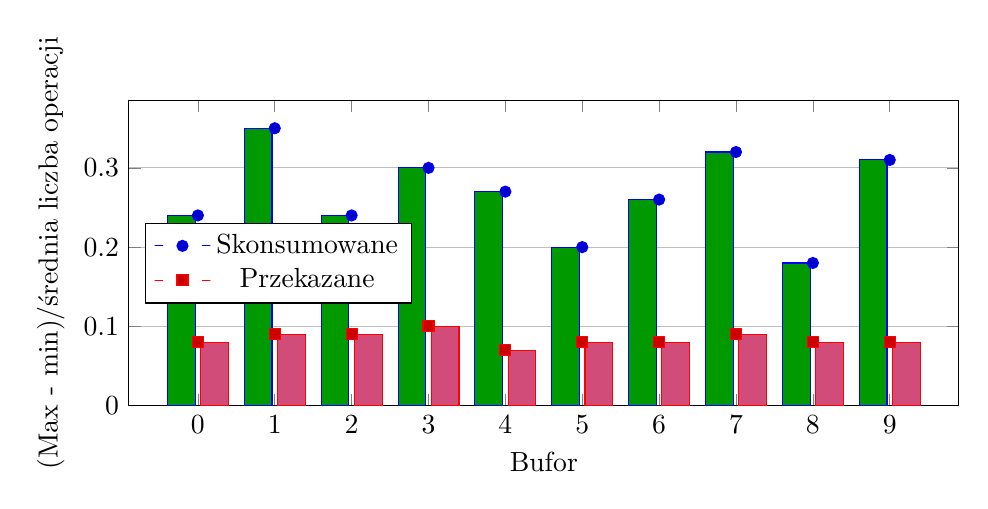
\begin{tikzpicture}
        \begin{axis}[
          width=\textwidth, height=0.45\textwidth,
          symbolic x coords={0,1,2,3,4,5,6,7,8,9},
          xtick=data,
          xlabel={Bufor},
          ylabel={(Max - min)/średnia liczba operacji},
          ymajorgrids=true,
          ymin=0,
          bar width=10pt,
          legend style={at={(0.02,0.6)},anchor=north west}
        ]
          \addplot+[ybar,fill=green!60!black,bar shift=-6pt] coordinates {
            (0, 0.24) (1, 0.35) (2, 0.24) (3, 0.30) (4, 0.27) (5, 0.20) (6, 0.26) (7, 0.32) (8, 0.18) (9, 0.31) 
          };
          \addplot+[ybar,fill=purple!70,bar shift=6pt] coordinates {
            (0, 0.08) (1, 0.09) (2, 0.09) (3, 0.10) (4, 0.07) (5, 0.08) (6, 0.08) (7, 0.09) (8, 0.08) (9, 0.08)                                                                                                 
          };
          \legend{Skonsumowane, Przekazane}
        \end{axis}
      \end{tikzpicture}
      \caption{Konsumenci - skonsumowane, a przekazane (Max - min)/średnia}
    \end{figure}

    \section{Wnioski}
      System dobrze radzi sobie z równoważeniem obciążenia w każdym testowanym przypadku. Zmniejszenie przestrzeni magazynowej nie zmniejsza przepustowości.
      Minusem jest skomplikowanie implementacji oraz duża liczba kanałów.


\end{document}
